\documentclass[11pt]{artuppax}

\usepackage[utf8]{inputenc}

%\setdefaultlanguage[variant=british]{english}
\setdefaultlanguage{french}
\setmainlanguage{french}
\setotherlanguage[variant=us]{english}

%\title{Demande d'accueil en délégation au CNRS}
\title{Dossier de demande d'un CRCT}
\author{G. Vallverdu}
\date{\today}
%\entete{Demande d'accueil en délégation au CNRS}
\entete{Dossier de demande d'un CRCT}
%\subentete{}
\HeaderUPPA

\usepackage[version=3]{mhchem}
%\setlength{\bibsep}{0pt plus 0.3ex}
%\geometry{a4paper, margin=2cm}
\usepackage{tabularx}

\usepackage[sectcntreset]{bibtopic}
\usepackage[numbers, sort&compress, super]{natbib}
\bibliographystyle{achemso_perso}

\usepackage[absolute,showboxes,overlay]{textpos}
\TPshowboxesfalse
\textblockorigin{2mm}{2mm}

\newcommand*{\bul}{~$\bullet$~\xspace}

\newcommand{\rubriq}[2]{
\vspace{2\parsep}
\begin{tikzpicture}
    \node[anchor=south west, font={\huge}, inner sep=0pt] at (0, 0) {\textsc{#1 :}};
    \node[anchor=south east, font=\LARGE] at (\textwidth, 0) {#2};
    \draw[ultra thick, black] (0, -.2) -- ++ (\textwidth, 0);
    %\node[fill=red] at (0, 0) {};
\end{tikzpicture}
\vspace{-8mm}}

\usepackage{url}
\usepackage{pdfpages}
\usepackage{fontawesome} % need xelatex
\usepackage{graphicx}

\usepackage{enumitem}
\setlist[itemize]{itemsep=2pt, topsep=0pt}
%\setlist{nosep}
%\setlength\itemsep{0pt}

\usepackage{titlesec}
\newcounter{subsec}[section]
\setcounter{subsec}{0}
\titleformat{\subsection}[hang]%
  {\bfseries\Large}%
  {\stepcounter{subsec}\thesubsec)}%
  {1ex}%
  {}%
  %[\vspace{-3ex}\rule{\textwidth}{0.75pt}]
\titlespacing*{\subsection}{0ex}{2ex}{0ex}

\titleformat{\subsubsection}[hang]{\bfseries}{}{0ex}{}
\titlespacing*{\subsubsection}{0ex}{0ex}{-1ex}


\fancypagestyle{titlepage}{%
        \fancyhead{}%
        %\fancyhead[C]{\includegraphics[height=2cm]{\@uppalogo}}
        \fancyfoot[R]{{}}%
        \fancyfoot[L]{}%
        \fancyfoot[C]{%
            {\color{black} UNIVERSIT\'E DE PAU ET DES PAYS DE L'ADOUR}%
            \begin{tikzpicture}[overlay, remember picture]
                \draw[thick, black] ($(current page.south west) + (0,1cm)$) --
                    ($(current page.south east) + (0,2cm)$);
            \end{tikzpicture}%
        }
    }

\renewcommand{\maketitle}{%
    \thispagestyle{titlepage}
    \singlespacing
    \begin{center}
        \parbox{.33\textwidth}{\includegraphics[height=2cm]{logotype_iprem}}
        \parbox{.33\textwidth}{\centering 
\includegraphics[height=2.5cm]{LogoUPPAcouleurRVB}}
        \parbox{.33\textwidth}{\hfill\includegraphics[height=2.2cm]{CNRS}}

        \vspace*{\stretch{1}}

        {\Huge\bfseries\setlength{\baselineskip}{1.2\baselineskip}%
        %Dossier de demande d'accueil en délégation au CNRS
        Dossier de demande d'un congé pour recherches ou conversions thématiques
        \par}

        \vspace{4ex}

        {\LARGE Germain VALLVERDU}

        {\Large IPREM - UMR 5254}

        {\Large\itshape\today}

    \end{center}
    \vspace*{\stretch{1}}
    }

% ------------------------------------------------------------------------------

\begin{document}

%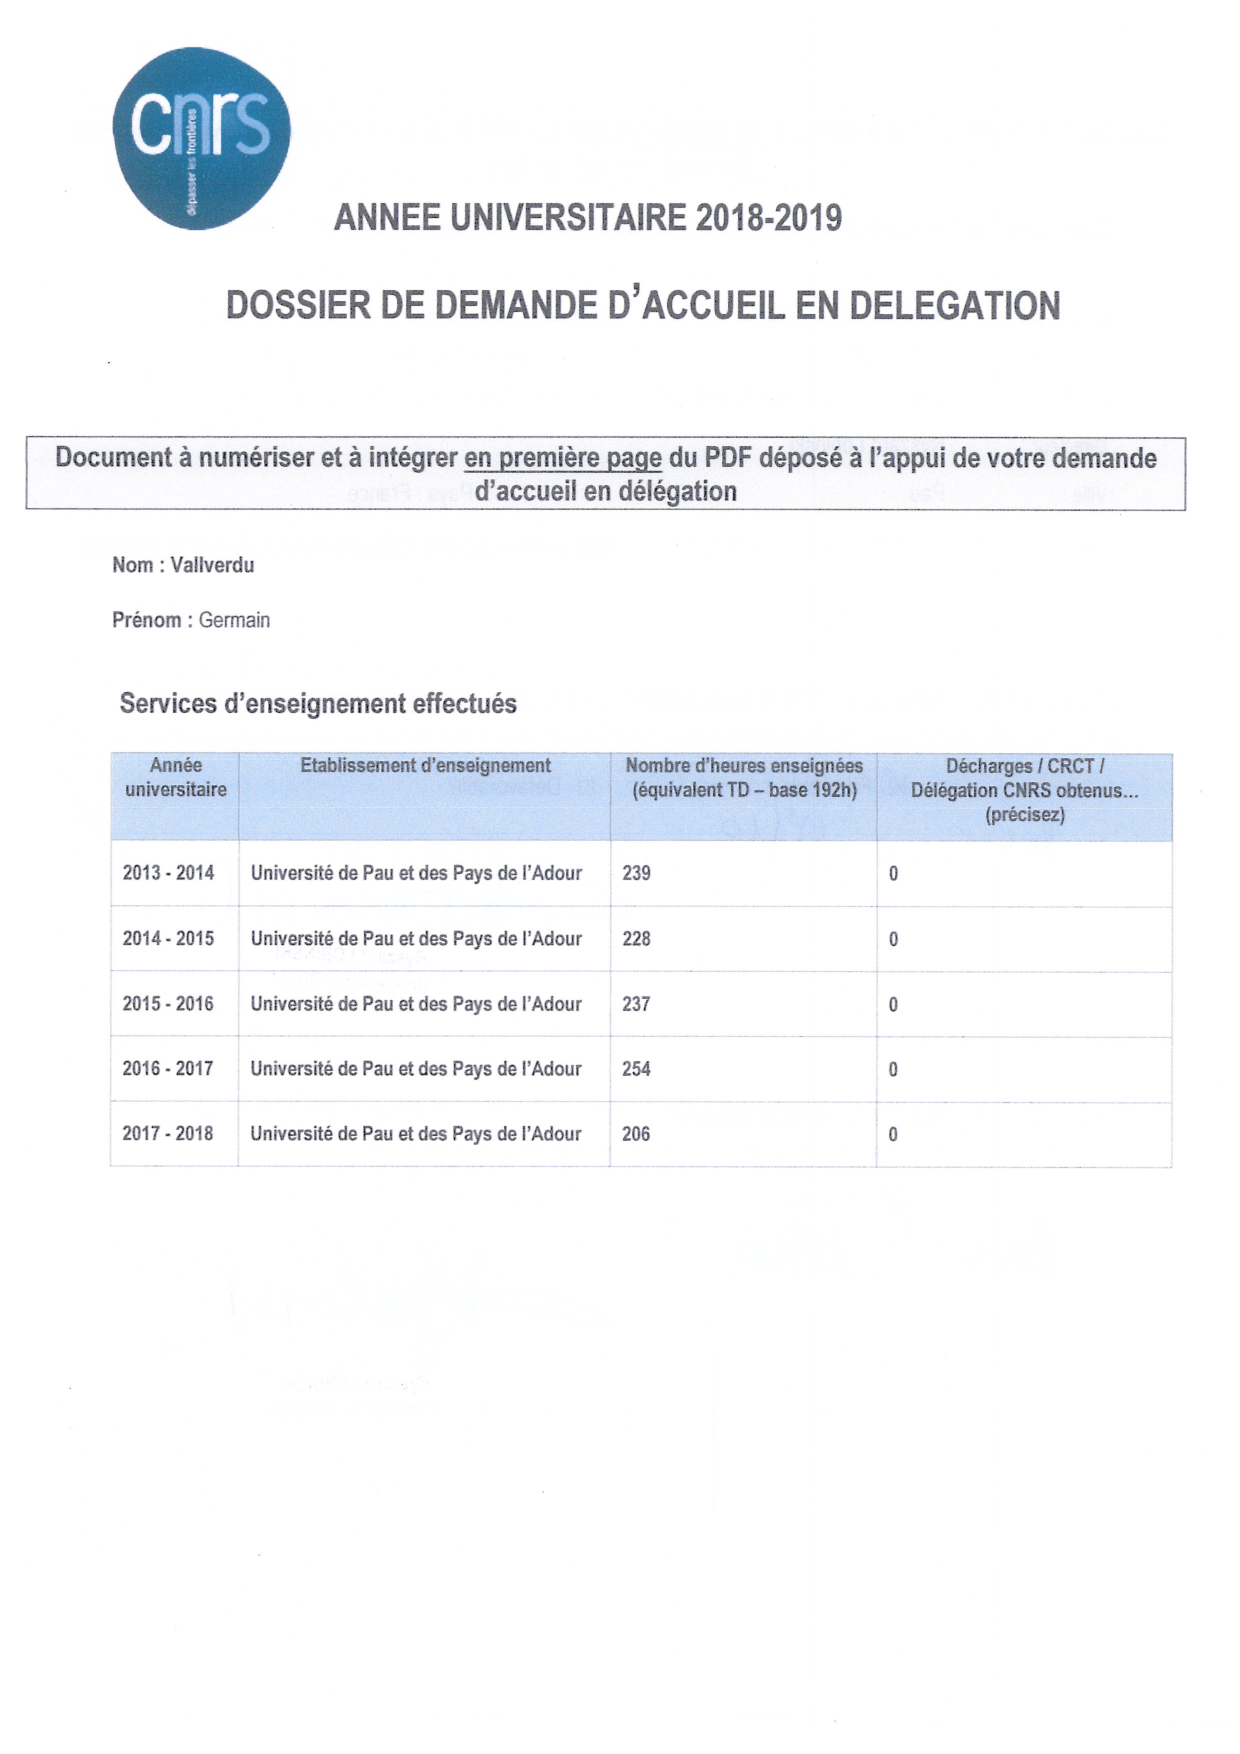
\includepdf[pages=1,scale=1]{formulaire.pdf}
%\includepdf[pages=2,scale=1, angle=180]{formulaire.pdf}

\maketitle

\newpage
\setcounter{tocdepth}{1}
\tableofcontents

\newpage

%\addcontentsline{toc}{section}{Curiculum Vitae court}

\includepdf[scale=1]{../cv-en-short.pdf}

%\section{Curiculum Vitae}

%\vspace*{5mm}
\begin{center}
    \LARGE
    \textsc{Curiculum Vitae}
\end{center}
\vspace*{10mm}
\addcontentsline{toc}{section}{1. Curiculum Vitae}

	\begin{textblock*}{60mm}(12cm,6cm)
	    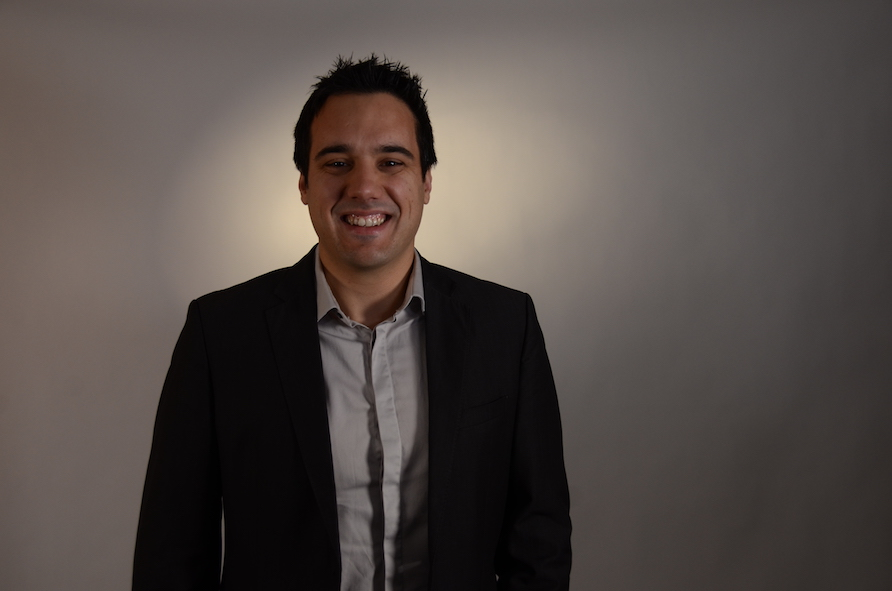
\includegraphics[height=4cm]{gvallver}
	\end{textblock*}


\textbf{\large Germain \textsc{Vallverdu}} \\
Nationalité française \\
Né le 10 Août 1983 à Perpignan (Pyrénées orientales) \\
Marié, 2 enfants


\faEnvelope{} IPREM\\
Technopôle Hélioparc\\
2 avenue du Président Pierre Angot\\
64053 Pau Cedex 9\\
\faPhone{} 05 59 40 78 51\\
\faAt{} germain.vallverdu@univ-pau.fr \par

$\vcenter{\hbox{
\includegraphics{../img/iD-icon}}}$ \url{orcid.org/0000-0003-1116-8776}\\
\faGithub{} \url{@gvallverdu - https://github.com/gVallverdu/}\\
\faGlobe{} \url{http://gvallver.perso.univ-pau.fr}

\singlespacing
\rubriq{Fonctions}{\faBlackTie}

\begin{description}
	\item \textbf{Octobre 2010 \faArrowCircleORight{} Aujourd'hui} \hfill \textit{Maître de conférences}
	\begin{itemize}
		\item Chimie théorique et simulation numérique. Surfaces, interfaces, couplage expérience-théorie.
		\item Université de Pau et des Pays de l'Adour
	\end{itemize}

	\item \textbf{2009 \faArrowCircleORight{} 2010} \hfill \textit{Chercheur-Ingénieur}
	\begin{itemize}
	    \item Développement et implémentation d'un modèle mésoscopique pour
	    l'étude de la propagation d'ondes de chock réactives.
		\item CEA - DAM Île de France.
	\end{itemize}

	\item \textbf{2006 \faArrowCircleORight{} 2009} \hfill \textit{Allocataire Moniteur}
	\begin{itemize}
	    \item Étude théorique de processus photophysiques dans des
		protéines fluorescentes.
		\item Université Paris Sud 11, Laboratoire de Chimie Physique, Orsay
	\end{itemize}
\end{description}

\newpage
\rubriq{Formation}{\faGraduationCap}

\begin{description}
	\item \textbf{16 Juillet 2009 \bul Soutenance de thèse}
	\begin{description}
		\item \textbf{Titre : } Étude théorique de processus photophysiques dans des
		protéines fluorescentes.
		\item financement MNRT, mention très honorable.
		\item \textbf{Composition du jury : }
		\begin{itemize}
			\item M. David Perahia (Directeur de recherche, IBBMC, Université Paris-Sud 11),
				\textit{président}
			\item M. Xavier Assfeld (Professeur, Université Henry Poincaré, Nancy),
			\textit{rapporteur}
			\item M. Daniel Borgis (Directeur de recherche, ENS Paris), \textit{rapporteur}
			\item M. Olivier Parisel (Directeur de recherche, lCT, Université Paris 6)
			\item Mme Fabienne Mérola (Directeur de recherche, LCP, Université Paris-Sud 11)
			\item Mme Isabelle Demachy (Professeur, LCP, Université Paris-Sud 11),
				\textit{directrice de thèse}
		\end{itemize}

		\item \textbf{Disponible sur Thèse en ligne}
			\begin{itemize}
				\item \url{http://tel.archives-ouvertes.fr/tel-00431879/fr/}
			\end{itemize}
	\end{description}

	\item \textbf{2006 - 2009 \bul Doctorat : Allocataire Moniteur à l'université Paris-Sud 11}
	\begin{itemize}
		\item[] Travaux de recherche effectués dans le Laboratoire de Chimie Physique,
		UMR 8000, financement MNRT, mention très honorable.
		\item[] Enseignements effectués à l'IUT de mesures physiques d'orsay.
	\end{itemize}

	\item \textbf{2003 - 2006 \bul Magistère de Physico-Chimie Moléculaire}
	\begin{description}
		\item Université Paris-Sud 11 et Ecole Normale Supérieure de Cachan.
	\end{description}

	\item \textbf{2004 - 2006 \bul Master de Physico-Chimie Molécualire}
	\begin{description}
		\item Université Paris-Sud 11, mention Très Bien.
	\end{description}

	\item \textbf{2003 - 2004 \bul Licence de Chimie Physique}
	\begin{description}
		\item Université Paris-Sud 11, mention Très Bien.
	\end{description}

	\item \textbf{2001 - 2003 \bul Classes préparatoires aux grandes écoles}
	\begin{description}
		\item Lycée François Arago (Perpignan), classes PCSI - PC.
	\end{description}

\end{description}

\onehalfspacing

% ------------------------------------------------------------------------------

\newpage

\rubriq{Activités d'enseignement}{\faPencil}
\addcontentsline{toc}{section}{2. Activités d'enseignement}
\stepcounter{section}

\subsection{Détails des enseignements}

Depuis mon recrutement en septembre 2010 à l'Université de Pau et des Pays de l'Adour (UPPA),
je suis rattaché au département
Chimie de l'UFR Sciences et Techniques de Pau où j'effectue l'essentiel de mon service.
Il s'agit d'enseignements de chimie-physique ou de chimie générale dont voici une
liste représentative:
\begin{itemize}\singlespacing
    \item Atomistique, L1 Physique-Chimie, Cours (9.5 HETD) /TD (10.5 HETD)
    \item États de la matière, L1 Physique-Chimie, TD (10.5 HETD)
    \item Atomistique et liaisons chimiques, L2 Chimie et Physique-Chimie, TD (19.5 HETD)
    \item Outils pour la symétrie moléculaire, L2 Chimie, Cours (9.5 HETD) / TD (10.5 HETD)
    \item Outils informatiques pour les sciences de l'ingénieur, L1, Cours/TD/TP (27 HETD)

    \item Travaux pratiques de techniques de séparation et d'analyse, L2 Chimie et Biologie (20 HETD)
    \item Travaux pratiques de catalyse chimique, L2 Chimie (20 HETD)
    \item Travaux pratiques de thermochimie et cinétique chimique, L2 Chimie (20 HETD)
    \item Travaux pratiques de structure et réactivité des molécules, L3 Chimie (16 HETD)

    \item Structure électroniques des solides, M1 Chimie et Physico-Chimie des Matériaux, TD (10.5 HETD).
\end{itemize}

Dans ce qui suit je présente les enseignements qui sortent des sujets classiques de
chimie et de chimie-physique, ou, dans lesquels une pédagogie spécifique a été mise en
œuvre. Un aspect transverse sur les points ci-dessous est l'utilisation avancée des technologies
de l'information et de la communication pour l'enseignement. Dans ce cadre, je participe
régulièrement au développement de la plateforme \textit{moodle} de l'UPPA\footnote{\url{https://elearn.univ-pau.fr/}}.

\subsubsection{Apprentissage par projets ou problèmes}

L'apprentissage par projets ou problèmes (APP) fait partie de ce que l'on appelle un mode
de pédagogie active dans lequel l'étudiant est acteur de son apprentissage. Dans un
enseignement sous forme APP, les étudiants travaillent en groupe sur un
problème (ou la réalisation d'un projet) dont la résolution implique des
notions qu'ils n'ont pas encore acquises et constituent les objectifs pédagogiques d'apprentissage.
C'est donc à eux d'acquérir ces notions, notamment au travers de documents fournis par les
enseignants. En plus de l'acquisition de ces savoirs, cette méthode permet de développer des
compétences transversales de travail collaboratif et de gestion de projets.
Ce type d'apprentissage a été mis en œuvre sur deux modules de la licence
de physique-chimie. Dans les deux cas, le cours est adossé à une plateforme en ligne,
de type \textit{moodle}, permettant de gérer la formation, les contenus et les livrables
des étudiants.

Premièrement, une activité de ce type a été proposée aux étudiants en préambule du module
"états de la matière" en L1 Physique-Chimie.
L'objectif était de découvrir les différents types de forces intermoléculaires et la notion
d'émulsion dans un contexte culinaire. Chaque groupe d'étudiants devait alors proposer une
recette originale de vinaigrette, ou sauce, en justifiant le choix des ingrédients sur
la base des propriétés des molécules choisies.

Deuxièmement, l'enseignement par projet a été employé dans le cadre d'un module de L2
chimie dont l'objectif est une première découverte de la recherche bibliographique. Les
étudiants, réunis en groupes, doivent réaliser un projet sur un sujet scientifique se rapportant à
l'actualité et présentant une controverse. Ils doivent alors faire les recherches
bibliographiques concernant les différentes thèses du sujet et restituer un document
présentant objectivement ces différents courant avec la bibliographie associée.

\subsubsection{Réseau Français de Chimie Théorique}

J'effectue des enseignements dans le cadre du label de Chimie Théorique, délivré
par le Réseau Français de Chimie Théorique. Ces enseignements concernent le pôle
sud-ouest du réseau dans lequel le label, initialement réservé aux étudiants en
M2, est, depuis 2016, ouvert à partir du M1. Cela permet, pour les étudiants qui
le souhaitent, d'accroitre la proportion des enseignements de chimie théorique sur l'ensemble
du master. Ce dernier point est possible grâce à la mutualisation de certains cours
sur les universités de Toulouse, Montpellier, Pau et Bordeaux. Les enseignements
que je dispense concernent la chimie théorique du solide :
\begin{itemize}
    \item Travaux pratiques d'introduction aux calculs de chimie quantique du solide avec VASP (2012, 2014, 2015, 2016, 2017).
    \item Cours, 8h : Theoretical approaches of surfaces and interfaces (2014 TCCM Toulouse, 2016 Pau)
\end{itemize}

\subsubsection{Outils pour la simulation numérique}

Je participe à la formation doctorale de l'ED 211, École doctorale des sciences exactes
et leurs applications, via deux modules de 10h qui sont proposés aux doctorants ou
aux personnels de l'université. L'objectif de ces modules est de former les participants
pour qu'ils soient en mesure de se servir d'un centre de calculs et d'utiliser avec
un esprit critique les codes mis à leur disposition. J'interviens principalement sur
ce deuxième aspect par une initiation à la programmation (Fortran ou Python) et une
sensibilisation à l'analyse numérique.

\subsubsection{Python, traitements et visualisation des données}

En complément de ce qui est proposé à l'école doctorale, j'ai créé un module dont
l'objectif est d'une part d'introduire le langage python ; et d'autre part, de
montrer comment s'en servir pour traiter ou visualiser des données. Ce module
est ouvert à l'ensemble des composantes de l'UPPA et fait l'objet d'une
intervention spécifique
à l'IAE de Pau pour les étudiants en M2 Chargé d'études économiques et de marchés (12 heures de cours).
Un projet est en cours pour ouvrir ce module sous la forme d'une formation à distance,
pour, à terme, le proposer dans le cadre du PIX ou dans le catalogue de la formation continue de l'UPPA.
Cette étape intermédiaire pourrait conduire à proposer ce cours sur
la plateforme FUN (France Université Numérique) en complément des cours déjà existant sur
le langage python.

\subsubsection{Documentation et bibliographie}

Dans le cadre du Master Métiers de la traduction et de la documentation de l'UFR Lettres,
langues, sciences humaines, j'ai effectué une intervention de 25 HETD jusqu'en 2016 dans
le module de documentation. L'objectif de cette intervention
était, d'une part, de confronter des étudiants littéraires à la documentation scientifique
et technique
et d'en présenter les spécificités ; et d'autre part, de former les étudiants à
l'utilisation d'outils de documentation tel que Zotero\footnote{https://www.zotero.org/}.
L'enseignement était effectué
essentiellement sous la forme d'un projet de documentation en lien
avec le projet de terminologie de la partie traduction du Master.

Sur ce thème de la documentation, je co-anime également un atelier à destination des
doctorants en première année dont l'objectif est de présenter l'utilisation de Zotero
et de \LaTeX{} pour la bibliographie.

\subsection{Vulgarisation et animations scientifiques}

Depuis mon doctorat, je participe ou organise des animations de vulgarisation
scientifique à destinations de publics scolaire ou pour tout public.

En lien avec mes activités de recherche en chimie théorique, j'ai proposé plusieurs
\textit{café des sciences} sur le thème de la mécanique quantique. Il s'agissait de faire
découvrir les aspects non usuels du monde microscopique et de replacer dans
leur contexte historique les différents modèles qui ont conduit au développement
de cette science. Ces animations permettent également de faire le lien avec la
plateforme instrumentale disponible à l'IPREM et en particulier la spectroscopie
de photoélectrons à rayonnement X ou le microscope à force atomique.

La conception de ces interventions a conduit à la création d'un jeu, type
\textit{jeu de l'oie}, mettant en œuvre quelques principes de mécanique quantique
tels que la quantification de l'énergie ou l'aspect probabiliste de cette théorie.
Il a été présenté en parallèle du Tic-Tac-Toe quantique (ou morpion quantique) proposé par
Allen Goff\footnote{Goff, Allen (2006). "Quantum tic tac toe: A teaching metaphor for superposition in quantum mechanics" American Journal of Physics. 74 (11): 962–973}.

\begin{btSect}{../bib/com_vulg}
    \singlespacing
    \setlength{\bibsep}{2pt plus 0.3ex}
    \textbf{Conférences, café des sciences}
    \vspace{-5mm}
    \btPrintAll
\end{btSect}

Depuis 2013, j'organise pour le département de Chimie de l'UFR Sciences et Techniques
de Pau deux journées d'accueil d'élèves du collège ou du lycée dans le cadre de la
fête de la science. L'objectif est d'accueillir ces élèves dans les salles de travaux
pratiques de l'université et de leur faire découvrir à la fois l'environnement
universitaire et quelques notions de chimie amusantes autour d'ateliers pratiques
lors desquels  les élèves manipulent. Chaque année nous recevons
une dizaine d'établissements pour environ 200 élèves. L'animation de ces ateliers
est assurée par des chercheurs, enseignants-chercheurs, ingénieurs et doctorants
de l'IPREM, ces interventions pouvant être validées dans le cadre de la formation
doctorale.

Ces animations ont donné lieu à la conception de trois ateliers :
\begin{itemize}
    \item Chimie et couleur: Mise au point et utilisation d'une échelle de couleurs
    pour déterminer le pH de produits de la vie courante.
    \item Synthèses de molécules olfactives : Synthèses rapides, en tubes à essai, de
    quelques esters aux propriétés olfactives.
    \item Identification d'une substance inconnue : Il s'agit d'une démarche d'investigation
    dans un contexte fictif d'identification de stupéfiants. À l'aide des tests chimiques
    proposés, les élèves doivent identifier six poudres blanches. Les tests sont ceux
    proposés par le \textit{National Institute of Justice (US)}.
\end{itemize}

% ------------------------------------------------------------------------------

\rubriq{Activités de recherche}{\faGear}
\addcontentsline{toc}{section}{3. Activités de Recherche}
\stepcounter{section}

\subsection{Encadrement doctoral}

Depuis mon recrutement j'ai participé à l'encadrement des thèses de
Lucile Martin (2010-2013), Émilie Guille (2011, 2014) et
Ambroise Quesne-Turin (2014-2017).

\textbf{Émilie Guille (2011-2014)} :
L'école doctorale ED211 et l'UPPA m'ont accordé une co-direction
à hauteur de 40\% avec le Pr Isabelle Baraille pour cette thèse.

Cette thèse a concerné l'étude de l'interface entre une électrode et un électrolyte
solide. Ce type d'électrolyte est utilisé pour contourner les problèmes de sécurité
inhérents aux électrolytes liquides dans des microbatteries au lithium. L'électrolyte
étudié était le \ce{Li_xPO_yN_z} (LIPON) qui présente une structure amorphe. La plus
longue partie de la thèse fut consacrée à l'identification de motifs représentatifs de
la structure du LIPON par comparaison de résultats expérimentaux et théoriques :
spectres IR, Raman, XPS. Le modèle a ensuite été utilisé pour étudier l'interface
entre le LIPON et une électrode modèle de silicium.

\subsection{Encadrement d'étudiants en M2 Recherche}

Depuis 2013 j'ai encadré 6 étudiants en Master 2 chimie et physico-chimie des matériaux,
spécialité recherche. 4 d'entre eux ont travaillé sur des sujets mixtes couplant expériences
et théorie en collaboration avec un expérimentateur de l'IPREM spécialiste de la caractérisation de
surface.

\begin{tabularx}{\textwidth}{lllX}
\hline
Nom de l'étudiant & année & taux & sujet \\
\hline
Marie Minvielle & 2013 & 50\% & Étude de l'adsorption de sondes gazeuses à la surface de
                                matériaux d'électrode positive: couplage expérience/théorie \\
Dimitri Del Pianta & 2014 & 50\% & Étude des processus d'insertion dans les matériaux
                                   d'électrode positive pour microbatteries au sodium \\
William Lafargue-Dit-Hauret & 2015 & 100\% & Étude théorique de la conductivité ionique à
                                     l'interface
                                     électrode/électrolyte solide: Application au système
                                     LiPON/Si\\
Youn Charles-Blin & 2016 & 50\% & Étude de la réactivité de surface de matériaux d'électrode
                                  modèles de la famille des oxydes de lithium lamellaire:
                                  approche couplée expérience/théorie\\
Amine Bekkali & 2017 & 50\% & Une étude via un couplage expérience-théorie des déplacements
                              chimiques en spectroscopie photoélectronique à rayonnement X\\
Guillaume Fradet & 2017 & 50\% & Calculs de spectres Infra Rouge.\\
\hline
\end{tabularx}

\subsection{Participation à un comité de sélection}

En 2013, j'ai participé au comité de sélection pour le recrutement d'un Maître de
conférence en section CNU 33 et 31. Le profil du poste concernait la
Physico-chimie des matériaux appliquée aux surfaces / interfaces.

\subsection{Projets}

\begin{itemize}
    \item Soumissions de projets de Demande d'Allocation de Ressources Informatiques (DARI)
    \begin{itemize}
        \item 2017 - 1 000 000 heures scalaires
        \item 2016 - 400 000 heures scalaires
        \item 2015 - 200 000 heures scalaires
        \item 2014 - 200 000 heures scalaires
        \item 2013 - 150 000 heures scalaires
    \end{itemize}
    \item 2016 - participation à la rédaction du Projet ANR INGROwTH (Rejeté à la deuxième étape).
\end{itemize}


\subsection{Research Activities}

My research activities on the last five years concern the development of new methods and
computational strategies at different time or space scales, applied to the investigation
of complex systems. The common thread of my activities is the strong interaction
with experimentalists and the will to address the considered issues in a complementary way,
each discipline shedding light on one specific facet of the question. Moreover, a special
attention is given to the accurate description of the interactions between the various objects of interest:
between molecules, between a molecule or an aggregate and one surface of a material, or
at the interface between two materials. On a computational point of view, that means to
be able to set up relevant models and to use the right computational methods to reach the
more accurate description that keep the whole study tractable.

Two main applications
were explored. First, electrode or electrolyte materials for lithium batteries. The IPREM
institute is one of the founders of the French Research Network on Electrochemical Energy
Storage (RS2E)\footnote{\url{http://www.energie-rs2e.com/}}. In that scope we investigated
electrode materials and in particular the processes that take place at the interface between
the electrode and the electrolyte. This was done through the PhD works of Lucile Martin
(2010-2013), Émilie Guille (2011- 2014), for which the doctoral school ED 211 give me
the opportunity to be co-director, and Ambroise Quesne-Turin (2014-2017). The full control
of interface phenomenon is crucial in the development of efficient lithium batteries as
they are directly linked to the aging and the capacity fading of the device. Second, more
recently, we considered the molecular characterization of complex matrices and in particular
the chemical and physical properties of the heavy part of crude oil. This research activity
takes place in the scope of a common laboratory, C2MC\footnote{Complex Matrices Molecular
Characterization \url{https://c2mclab.wordpress.com/}}
between the university of Pau, the university of Rouen, the CNRS and Total. Here, we attempt
both to understand the aggregation mechanism of asphalten molecules and to get a more
accurate knowledge of the chemical structure of these molecules.

\subsubsection{Solid-Solid interfaces in Lithium microbatteries}

During the PhD of Lucile Martin we investigate the solid-solid interface in CuO, a conversion
material. This material is used as positive electrode in micro-battery devices whose
thickness do not exceed several micrometers and the surface several millimeters square.
In such compounds, the insertion of \ce{Li+} cations in the electrode involves a complete
reduction of the transition metal into a composite electrode described as nano-sized
metallic particles embedded in a \ce{Li_xO} matrix.
In such system, there is a huge proportion of interfaces and interfacial phenomenon play
a dominant role and the efficiency of the targeted properties are directly linked to
the processes taking place at the interface. Nevertheless, reliable
and precise data whether at the structural or chemical level are often obtained with difficulty
from experimental techniques. Their low thickness, their possible reactivity and their difficulty
of access from bulk or surface techniques explain that few experimental works report data on
solid/solid interfaces. Theoretical approaches are then interesting tools in order to investigate
such system.

\begin{figure}[h]
    \centering
    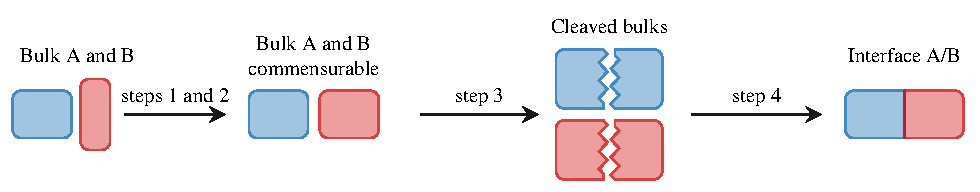
\includegraphics[width=.8\textwidth]{img/cycleThermo}
    \caption{Successive steps leading to an interface model from two bulk phases A and B.}
    \label{fig:cycleThermo}
\end{figure}

In that scope we developed a computational strategy in order to build solid-solid interface models,
figure \ref{fig:cycleThermo} and to investigate the thermodynamic properties of such systems. Indeed,
the relative stability of such interfaces is correlated to the chemical composition of the interface
and in order to describe that specificity a grand canonical approach is needed. In that thermodynamic
ensemble, the stability of the interface models is given as a function of a chemical potential. We
choose to use the chemical potential of \ce{Li+} which can be directly linked to the voltage against
a \ce{Li|Li+} electrode that is of high interest in the case of lithium battery applications. An
example of one model, the \ce{Li2O-Cu} interface is depicted figure \ref{fig:interfaces}.

In order to suggest the nanostructuration of the electrode material along the electrochemical
cycle, we computed the works of adhesion between the different systems. The comparison between the
different possibilities allow us to suggest a nanostructuration in agreement with tunneling electron
microscopy results at the beginning and at the end of the \ce{Li+} insertion. We thus suggested the
scheme depicted figure \ref{fig:interfaces} as the general case.

\begin{figure}[h]
    \centering
    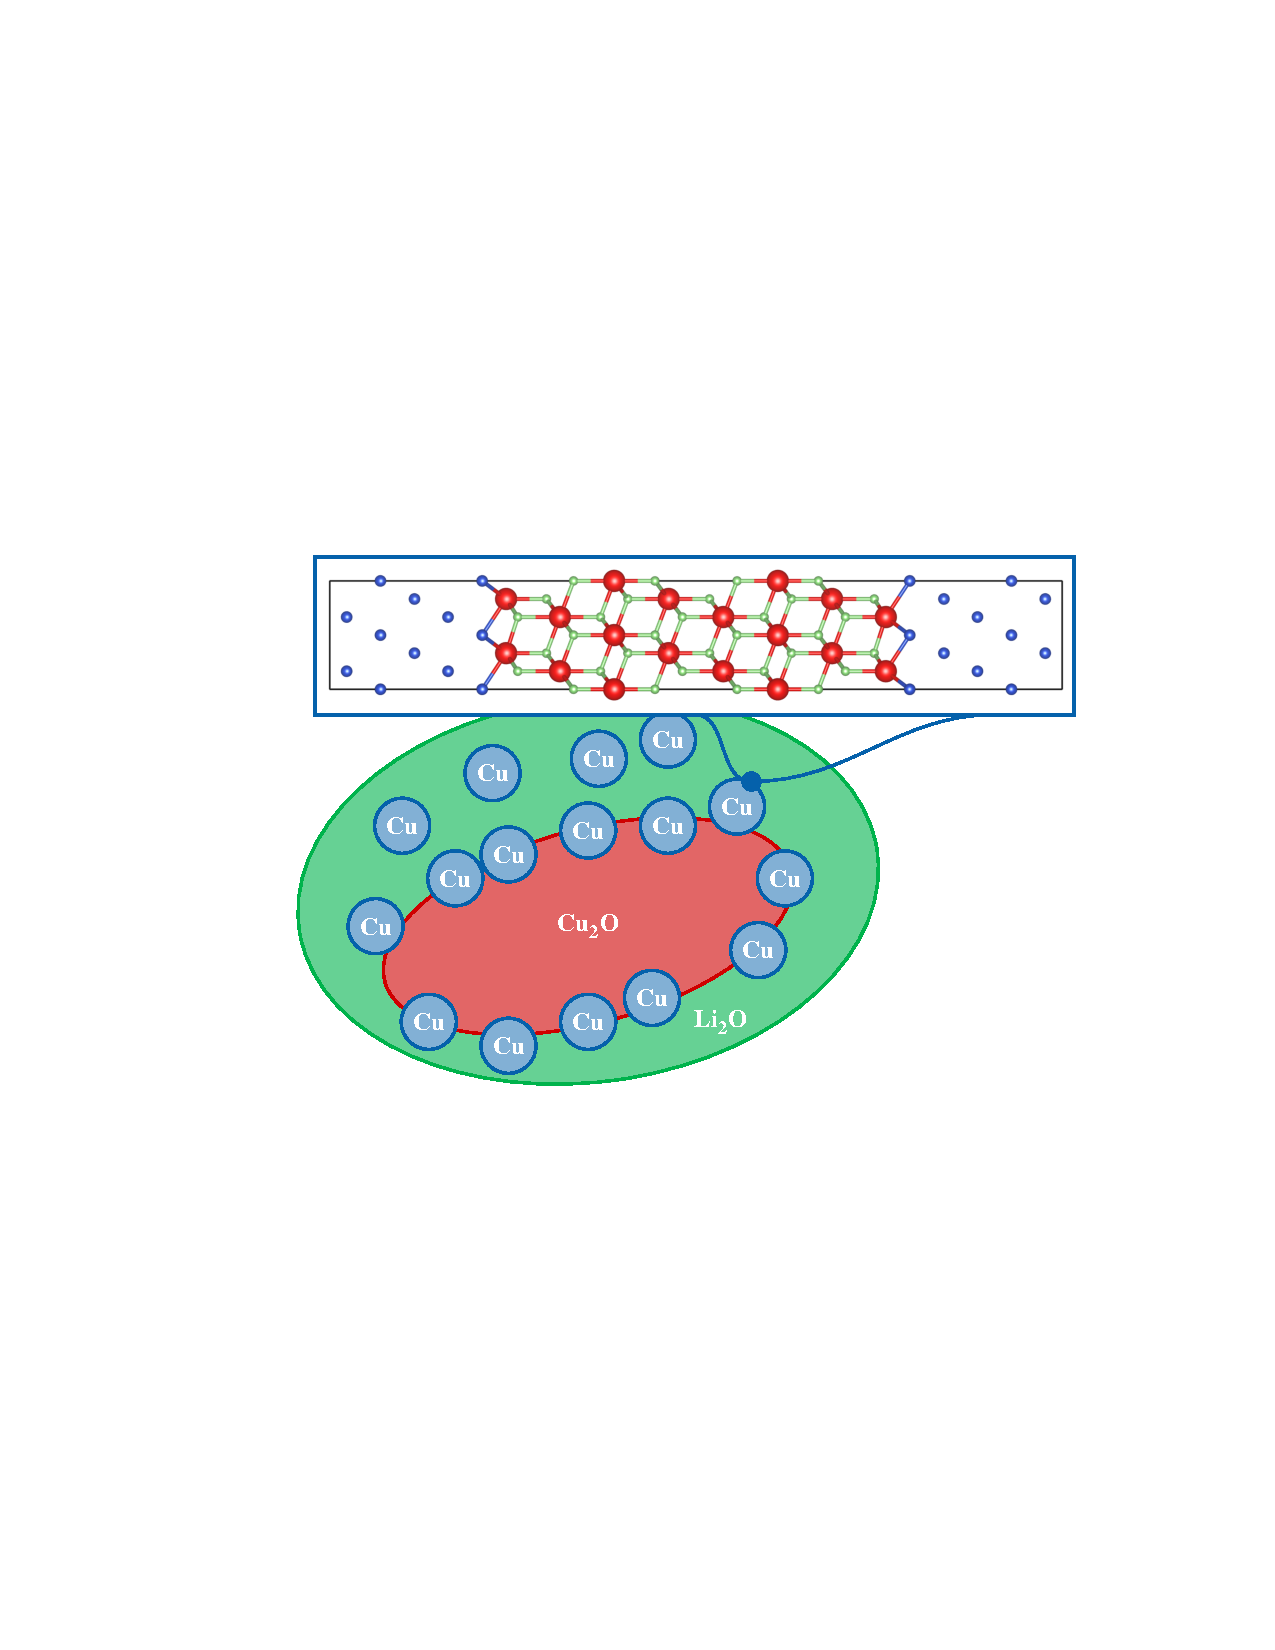
\includegraphics[width=.5\textwidth]{img/interfaces}
    \caption{This picture presents the suggested nanostructuration of the CuO electrode during
    the electrochemical cycle and focus on an example of a model for the solid-solid, \ce{Li2O-Cu},
    interface.}
    \label{fig:interfaces}
\end{figure}

\subsubsection{Electrode-Electrolyte interface with a solid electrolyte}

In the continuation of the investigation of solid-solid interfaces, we considered the interface
between a solid electrolyte \ce{Li_xPO_yN_z} (LIPON) and an electrode. On a theoretical point of
view, the challenge of this study lies both in providing an accurate description of the LIPON structure
and in the calculation of reliable spectroscopic properties on this compound in order to compare them
to the experimental data available. The LIPON consists in an amorphous structure with more or
less long chains of \ce{PO_4^{3-}} tetrahedron doped by nitrogen. Available experimental data are
mainly spectroscopic data, that are Raman spectra and X-Ray photoemission spectroscopy (XPS) core peaks
spectra.

\begin{figure}[h]
    \centering
    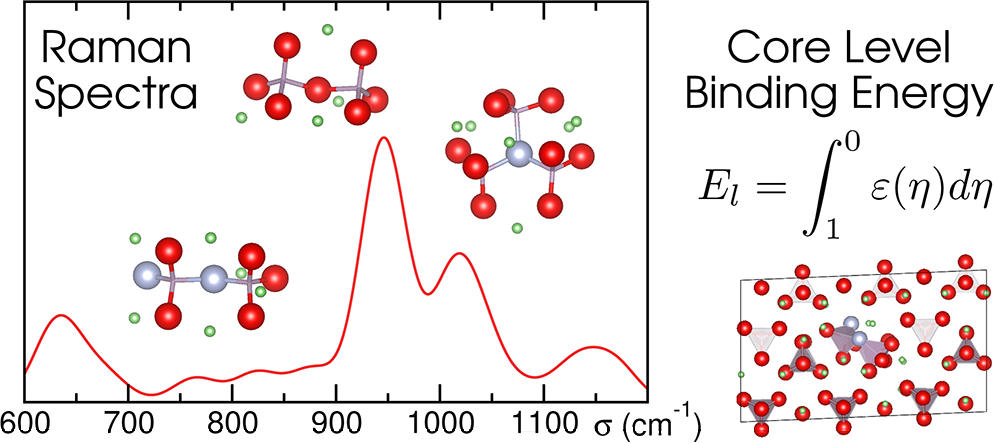
\includegraphics[width=.6\textwidth]{img/lipon}
    \caption{Examples of aggregates and bulk periodic systems investigated in order to identify recurrent
    pattern in the amorphous structure of LIPON. On the left, the main contribution of each aggregate
    to the Raman spectra are highlighted.}
    \label{fig:lipon}
\end{figure}

During the PhD of Émilie Guille, we first attempted to identify recurrent patterns in the amorphous
structure of LIPON. We compute the XPS bending energies of N 1s, O 1s and P 2p core peaks
and Raman spectra of both bulk periodic systems and aggregates extracted from a molecular dynamics
annealing. This allowed us to suggest a possible existence of a monovalent coordination for the nitrogen
atoms in the phosphate aggregates, see figure \ref{fig:lipon}. This study, was the first one in the
laboratory, in collaboration with the experimentalists of the XPS platform, for which a direct
calculation of the XPS core peak was undertaken.

The identified aggregates were the used in order to build interface models between a silicon electrode and
the LIPON. The adhesion energies of the LIPON aggregates and the migration barrier of \ce{Li+} cations
at the interface were investigate as a function of the nitrogen rate. We highlighted the crucial role
of nitrogen in order to ease the migration at the interface.

\subsubsection{Surface reactivity of lithium oxides}

This research activity, still concern the phenomenon taking place at the interface. But here, we consider
the interface between an electrode material and an electrolyte and more precisely the surface reactivity
of the material. The considered materials belong to two main families. First, we investigated the lithium
layered oxides, among them, \ce{LiCoO2} being widely used as positive electrode in commercial cells.
Due to its high cost and toxicity, cobalt atoms are usually substituted by nickel or manganese atoms,
leading to the so-called NMC materials (\ce{LiNi_xMn_yCo_zO2}). Second, we considered the spinel
compounds \ce{LiMn2O4}, which is a promising compounds due to its high voltage stability. The
surface reactivity is investigated indirectly, following an original approach developed in the laboratory.
The approach consists in the adsorption of gaseous probes at the surface of the material, in controlled conditions,
followed by an XPS characterization of the adsorbed species in order to identify and quantify the adsorbed
species. Concomitantly, computational approaches allow us to
describe more precisely the electronic processes taking place after the chemisorption of the gaseous
probes. This study was done in collaboration with Laurence
Croguennec and Michel Ménétrier, from ICMCB who provides us several samples for experimental investigation.

\begin{figure}[h]
    \centering
    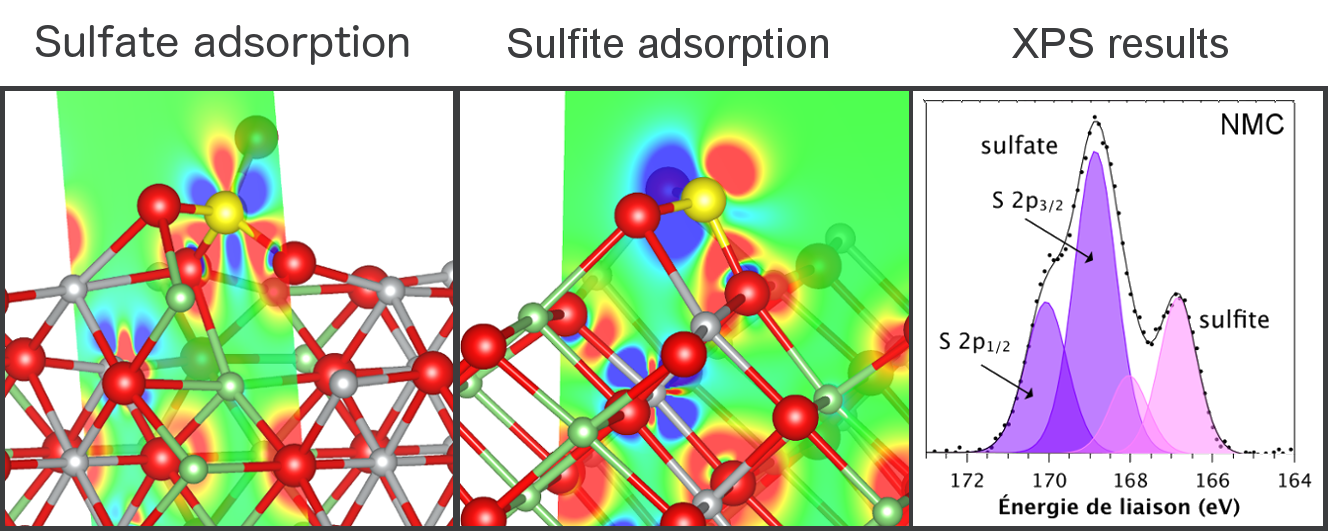
\includegraphics[width=.8\textwidth]{img/so2}
    \caption{\ce{SO2} adsorption on the surface of \ce{LiCoO2}: sulfate adsorption (left panel)
    sulfite adsorption (middle panel), S 2p XPS core peak after \ce{SO2} adsorption on
    \ce{LiNi_{1/3}Mn_{1/3}Co_{1/3}O2}(right panel). The color scale shows
    the difference between the converged electronic density and the sum of atomic densities
    (positive values are red).}
    \label{fig:SO2}
\end{figure}


The gaseous probe \ce{SO2} was used because of its high reactivity and allow us to probe the acidic sites
of the surface. Moreover, the S 2p XPS core peak presents a wide chemical shift scale which ease the
identification of the adsorbed species.
The chemisorption of \ce{SO2} leads to the formation of sulfite (\ce{SO3^{2-}}) or sulfate
(\ce{SO4^{2-}}) species, see figure \ref{fig:SO2}. The computational
results allowed us to describe two electronic processes associated to a redox or an acid-base reactivity
linked to the formation of sulfate or sulfite species, respectively. We considered the lamellar \ce{LiMO2}
(M = Ni, Mn, Co) and \ce{Li2MnO3} compounds and the spinel \ce{LiMn2O4} compound. This allow us to investigate
in details the role of the oxidation degree of the manganese atoms and the morphology of the material, on
the surface reactivity. The presence of \ce{Mn^{3+}} cations was associated to high miller index surfaces
and to the formation of sulfite species with an acid-base reactivity ; whereas the presence of
\ce{Mn^{4+}} cations, was associated to a higher and redox reactivity with the formation of sulfate species.

\subsubsection{Molecular characterization of complex matrices}

More recently, I have started to work on the molecular characterization of complex matrices and more
specifically on the molecular description and the chemical-physics properties of
crude oil. The complexity of such system comes with the diversity of the molecular species composing the
mixture, the exact composition being still not completely known. The whole species can be
described as a continuum, from a simple methane molecule to a large poly-cyclic
aromatic hydrocarbons substituted with several alkyl side chains.
In these first studies, the issue we would like to address
was to better understand the nano-aggregation of the high-molecular weight phases of crude oil and
in particular the asphaltene molecules. To that end, a series of classical molecular dynamics
simulation was undertaken.

\begin{figure}[h]
    \centering
    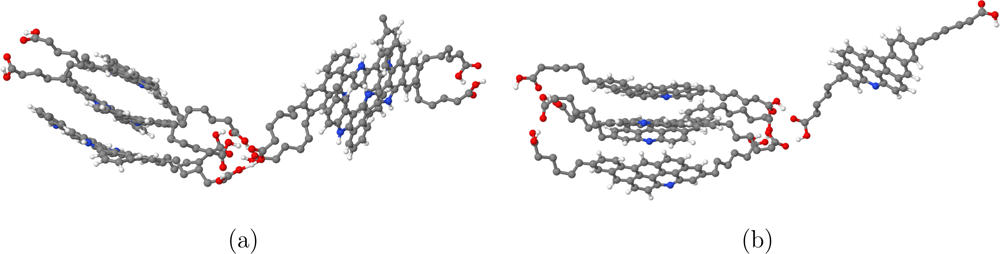
\includegraphics[width=.8\textwidth]{img/asphaltene}
    \caption{Snapshot from a molecular dynamics simulation (60 ns) of 5 asphaltene molecules in
    toluene at 298 K and 1 bar. The solvent is hidden. These snapshots illustrate the two interactions
    highlighted: the $\pi$-stacking between the aromatic nucleus and the hydrogen bonds between
    the side chains.}
    \label{fig:SO2}
\end{figure}

Both chemical and physical factors were taken into account. First, the chemical nature of the molecule
itself was considered by screening the
effects of the positions of heteroatoms such as nitrogen, oxygen or sulfur. Second, the role of
metalloporphyrins, who also make part of this crude oil fraction was considered and more
precisely the role of free base porphyrins and the vanadyl one. Finally, we
investigated the sensitivity of asphaltene molecules aggregation towards the thermodynamic
conditions, that is temperature and pressure. This studies allow us to identify and quantify
the two interaction types leading to the formation of nano-aggregates energy: the $\pi$-stacking
interactions and the formation of hydrogen bonds.
%It appears that the main chemical factors are the conjugated core
%size and the chain-end. The presence of porphyrins
%

\subsection{Production scientifique}

\singlespacing
\begin{itemize}
    \item 15 articles (with 2 under review)
    \item h-\textit{index} = 7\footnote{Sources : ISI Web Of Knowledge}
    \item 12.17 average citations per articles
    \item 146 citations (138 without self-citations)
    \item 11 conferences (with 7 in national congresses)
\end{itemize}

\begin{btSect}{../bib/articles}
    \subsubsection{Articles in international and peer reviewed journals:}
    \smallskip
    \btPrintAll
\end{btSect}

\begin{btSect}{../bib/com_perso}
    \subsubsection{Personal conferences}
    \smallskip
    \btPrintAll
\end{btSect}

\begin{btSect}{../bib/com_autres}
    \subsubsection{Conferences done by others}
    \smallskip
    \btPrintAll
\end{btSect}

\begin{btSect}{../bib/poster}
    \subsubsection{Posters}
    \smallskip
    \btPrintAll
\end{btSect}

\newpage
\onehalfspacing
\rubriq{Research project}{\faBook}
\addcontentsline{toc}{section}{4. Research Project}
\stepcounter{section}


\begin{btSect}{biblio}
The present demand relies on a research project in the IPREM institute which is described below. This project occurs at a special date for the university of Pau \& Pays Adour (UPPA) which has just succeeded in 2017 to the French Initiative of excellence I-Site. This success has led to the creation of the E2S project: Energy Environment Solutions\footnote{http://e2s-uppa.eu/en/index.html}. The core scientific domain of the project focuses on Environment and Energy and relies on strongly recognized laboratories supported by state-of-the-art equipment. This is a new challenge for UPPA which will define its future position at the European and international level. The current demand will allow me to take a full advantage of this high dynamic configuration.

The E2S project, provides a series of call for proposals in order to increase the scientific skills in the thematic of excellence and the international visibility of the laboratories. In particular, several chairs of excellence are supposed to start in the coming year in close interaction with my research activities. Simultaneously, I will apply for the current call of proposals of the young researcher program of the French National Research Agency (ANR JCJC 2018). The teaching vacation demanded will allow me to play a full part in this project and to contribute actively to the scientific program of the chairs. Finally, this will permit me to broaden my research skills and reach the require experience in order to apply for an HDR (Accreditation to Supervise Research).

The current project focusses on the study of the chemical reactivity using molecular dynamics simulations. The long-term objective is to describe dynamically the whole chemical-physics process by considering both the thermodynamic and kinetic aspects of the reactivity. To reach this objective, it is necessary to develop new methods able to describe the potential energy surface of the system in condensed matter.

\subsection{Context and objectives of the project}

Molecular dynamics simulation is an essential tool to gain insight into dynamical molecular processes of condensed matter at the atomic scale and is nowadays widely applied to a huge variety of systems from biological systems to oil mixtures. The accuracy of the simulations is directly associated to the parametrization of robust and reliable force-fields associated to the potential energy surface of the system.  Nonetheless, force-fields always require a trade-off between accuracy and computational cost. In consequence, the parametrization of a new force-fields needs to follow a robust procedure with well identified target properties and applications to ensure the quality of the model.

A variety of classical force-fields devoted to biological applications have been developed: GROMOS\cite{gromos}, AMBER\cite{amber} or OPLS\cite{opls1996}, among others. The development of these force-fields followed different strategies which lead to a large discrepancy in the parameters although the analytical potential energy functions are similar. This illustrates the difficulty of force-field parametrization. Indeed, because of the large number of parameters and the amount of target data the solution is highly underdetermined and parameters strongly correlated. Nonetheless, biological force-fields are successful and are able to describe numerous properties of biological systems. A reason of this success is that the available force-fields reproduce accurately the properties of a core set of a limited number of molecules such as amino acids, common solvent or nucleotides, that governs the chemistry of these systems.

In order to address the investigation of, for example, structure-based drug-design techniques, throw the screening of large pharmaceutical database, new general force-fields were developed\cite{gaff} and automatic force-field parametrization programs or platforms\cite{atb, prodrg}, provides facilities to obtain the parameters of a custom drug or substrate. This can be achieved following two strategies. The more usual, is based on the determination of atom types from the local environment of each atom of the molecule. Thanks to robust databases associating atom types and force constants, the parameters of the force-field are extracted for each term of the chosen potential energy function\cite{atb, prodrg}. The second strategy consists in determining the force-field parameters directly from \textit{ab initio} calculations. Recently \citet{zheng2016} proposed a new software, based on the Seminario method\cite{nilsson2003} which computes directly the required parameters from a subset of the Hessian matrix of the system.

Nevertheless, classical force-fields failed to describe the chemical reactivity. Indeed, the chemical bonds are defined at the beginning of the simulation and bond breakings are not allowed. To circumvent this issue, the ReaxFF force-field was developed by Adri van Duin, William A. Goddard, and co-workers at the California Institute of Technology\cite{reaxff2001}. ReaxFF replaces the explicit definition of bonds by a bond orders criteria, which allows continuous bond forming/breaking. Developed to be as general as possible, it has been parameterized and tested for hydrocarbon reactions, high-energy materials, or catalytic systems with transition metals. As a results, ReaxFF is an efficient intermediate computational method between \textit{ab initio} and classical molecular dynamics.

For the last ten years, a new class of potentials has been proposed by \citet{behler2007} which takes full advantages of the emerging technologies about machine learning algorithms. The aim of this new potentials is to provide an efficient method able to compute the energy and the forces acting on a system with a comparable accuracy as \textit{ab initio} calculations. In order to do that, \citet{behler2007} introduce a neural-network representation of the \textit{ab initio} potential energy surfaces. This approach makes possible molecular dynamics simulations of large systems (or long time scale), with high accuracy. A recent article\cite{behler2017} reviews a wide range of applications of this method. This new potential is intrinsically a reactive potential because it is only based on \textit{ab initio} calculations and does not need the explicit definition of chemical bonds. Nevertheless, the new bottleneck of the calculations is now the construction of the training set from which the neural network \textit{"learns"} the potential energy surface and consists in a large number of \textit{ab initio} calculations.

Using the above-mentioned strategies, in this project, I want to develop new force field (i) based on automatic generation, (ii) able to describe the reactivity and (iii) implemented with modern algorithms. The aim is to describe various properties such as transport, thermodynamic or catalytic properties. The target systems will be hydrocarbon systems in condensed matter with heteroatoms (O, N, S) and transition metal (Ni, V). In order to reach this objective, three steps are considered at more or less long term.

\subsubsection{Classical force-field}

\textbf{Task 1:}
This first step focuses on the development of a global strategy in order to obtain reliable and robust classical force-fields using an automated procedure. Several aspects will be combine to set up this strategy. First, the input data to build the force-field will be extracted from \textit{ab initio} calculations and in particular the Seminario method\cite{nilsson2003} will be used to compute the needed force constants. Next, we will take advantage of the strong and recognized experience of the laboratory on the molecular vibrational properties and IR or Raman spectra will be the target properties for the fit of the force-field parameters. Using, home made code, the vibrational properties would be considered at the harmonic or anharmonic levels using the highly efficient AVCI algorithm recently developed by \citet{odunlami2017, garnier2016}.

This task will be achieved by the validation of the force-fields against experimental data, using the data base of IR spectra built by the Pr John Shaw (University of Alberta)  and Dr Michaelian Kirk (University of Alberta) who collaborate with our laboratory on the investigation of crude oil systems.

\textbf{Task 2:}
The validated force-fields parameters will be stored in a consolidated data-base. As a result, the force-field parameters of a canonical basis set of small molecules could be constructed and then, used to compute parameters for larger or more complex molecules. This second step could be achieved from the implementation of modern statistical algorithm based on machine learning or deep learning algorithm. Two approaches could be considered. The first one would be based on the link between the topology of the molecule and the force-field parameters and compute interpolated parameters for new molecules. The second one would be based on the molecular fragmentation methods, in order to get the electronic structure and the Hessian matrix of the large molecules from the calculations of smaller ones\cite{he2014, collins2014}.

\subsubsection{Reactive and quantum force-field}

Using the force-fields obtained from Task 1 and 2, we will be able to describe the initial and final states of a chemical reaction. We need now to switch on reactive force-fields. Here the aim is to describe bonds forming/breaking accurately but with cheap calculations. Neural Network Potentials were recently used to investigate organic reactions\cite{gastegger20015} but the \textit{ab initio} calculations needed to build the training set are still a strong bottleneck.

\textbf{Task 3:}
Following the strategies of classical force-fields, we propose here to develop quantum force-fields, based on semi-empirical methods. The force constants used as parameters in classical force-field will be replaced by the parameters of the semi-empirical method which describe the ground state of the system.  This approach is a trade-off between the possibility to describe the efficiently the reactivity and the accuracy of semi-empirical methods. The strategy followed to achieve Task 1 and 2 and the acquired experience will be applied in this  Task with the new parameters.


\textbf{Task 4:}
In order to go further in the description of the quantum properties along the dynamic of the system, several improvements of the quantum force-fields developed in Task 3 could be done. In particular, in the case of open-shell molecular systems such as a metalloporphyrins or a metallic catalyst, a multi-reference or valence-bond approaches, based on the semi-empirical wavefunction would be implemented. The aims are to investigate a wide field of applications by considering excited states dynamics or electronic transfer.

\subsection{Project organization and means implemented}

In the IPREM institute, I am involved in two projects in line with the research priorities of the institute: The french research network electrochemical energy storage (RS2E) and the Complex Matrices Molecular Characterization (C2MC), the current project positioning itself, in this later one. Moreover, the present project topic is totally in line with the project under way of the university about Energy and Environment Solutions (E2S project).

This project will be supported by several researchers of the IPREM institute and a mathematician of the LMA laboratory (Laboratory of mathematics and their applications). Moreover, external collaborations with Pr John Shaw (University of Alberta, Canada) and Dr Michaelian Kirk (University of Alberta, Canada), will be helpful for the comparison with experimental data.

In the IPREM institute, Hugo \textsc{Santos-Silva} (Postdoc) expert in molecular dynamic simulations and specialist of crude oil investigations, will contribute to the new methods for the force-field parameters determination both on the development point of view and on the needed computational effort to obtain and validate the parameters. Didier \textsc{Bégué} and Isabelle \textsc{Baraille}, full professors in theoretical chemistry will contribute by their deep and recognized experience in\textit{ab initio} calculations and vibrational properties which will be used as target properties for the development of the new force-fields. Finally, Brice \textsc{Bouyssiere}, full professor in analytic chemistry and specialist of crude oil and molecular characterization will provide precious insight and valuable experimental data in order to investigate complex matrices.

The LMA laboratory, part of the IPRA institute (multidisciplinary research institute applied to petroleum engineering), will bring to the team the needed skills in statistical and probabilistic approaches in order to implement relevant machine learning algorithms.

The UPPA university provides various local and regional high performance calculations (HPC) and data storage facilities which will be used in this project. Moreover, the members of the team are accustomed to answer to the calls concerning national HPC facilities (several hundred of thousand hours by year on the four last years and one million hours last year). This expertise in HCP will be advantageously exploited to reach the objectives of the current project.

\subsection{Impact and benefits of the project}

The methods developed in the scope of this project will provide powerful tools in order to investigate complex systems applied to the energetic transition.

The first application of the method will be devoted to the investigation of complex matrices particularly in the case of petroleum chemistry. The aim is to establish a clear cartography of the molecule existing in crude oil and to determine the composition of such complex mixtures in order to get a better knowledge and understanding of their chemical and physical properties. In that scope, using our classical force-field we will investigate complex mixture by screening a wide range of molecules. Moreover, the reactive and quantum force-field will be useful to investigate the role of transition metal in the chemical reactivity inside these mixtures.

More generally, the force-field will be designed to investigate accurately the molecular interactions between organic systems and between organic and inorganic systems. This will open a wide field of research. This is of high interest in order to develop new catalyst, for example for the dehydrogenation of \ce{CH4} or \ce{H2S}; or to improve the efficiency of matrices for \ce{CO2} storage.

This project is in line with the SNR (National Strategy of Research) challenge about the energetic transition: A sustainable, green, secure and efficient energy. Its theoretical aspect agrees with the objectives of the sub-thematic about fundamental, exploratory and breaking research.

\singlespacing
\subsection*{References}
\setlength{\bibsep}{2pt}
\btPrintCited

\end{btSect}


\end{document}

% ------------------------------------------------------------------------------
% ------------------------------------------------------------------------------
% ------------------------------------------------------------------------------

\newpage
\singlespacing

\section{Fiche récapitulative}

\textbf{\large Germain VALLVERDU}

Né le 10 Août 1983 (34 ans), Marié, 2 enfants.

\begin{description}

%  \item \textbf{Formation :}
%
%    \begin{itemize}
%	\item Doctorat de Chimie Physique de l'Université Paris-Sud 11 (16/07/2009),
%	Mention Très Honorable.
%	\item Magistère de Physico-Chimie Moléculaire (2003-2006).
%	\item Master de Physico-Chimie Moléculaire (2004-2006), Mention Très-Bien.
%	\item Licence de Chimie Physique (2003-2004), Mention Très-Bien.
%	\item Classe préparatoire aux grandes écoles (2001-2003). \\
%    \end{itemize}

\item \textbf{Doctorat (2006-2009) :}
    \begin{itemize}
	\item \textit{Etablissement :} Université Paris-Sud 11
	\item \textit{Titre :} Etude théorique de processus photophysiques dans des
	protéines fluorescentes.
	\item \textit{Directeur de thèse :} Isabelle Demachy
	\item \textit{Laboratoire d'accueil :} Laboratoire de Chimie Physique - UMR 8000. \\
    \end{itemize}

  \item \textbf{Activités de recherche (2010-aujourd'hui) :}

    \begin{itemize}
	\item Post-doctorant au CEA dans le département de physique théorique appliquée, service
	de physique de la matière condensée.
	\item \textit{Sujet :} Développement de modèles mésoscopiques d'ondes de choc réactives dans un
	milieu hétèrogène.
	\item \textit{Encadrant :} Jean-Bernard Maillet
	\item \textit{Laboratoire d'accueil :} Laboratoire de détonique et de dynamique des matériaux - CEA. \\
    \end{itemize}

  \item \textbf{Production scientifique :}
    \begin{itemize}
	\item 14 articles dans des revues internationales à comité de lecture.
	\item 11 conférences (dont 7 dans des congrès nationaux).
	\item h\textit{-index}: 7
	\item 146 citations, en moyenne 12.2 citations par article
	\item \url{http://orcid.org/0000-0003-1116-8776} \\
    \end{itemize}

% Web of Knowledge : Germain Vallverdu:
% 12 publications
% h-index : 7
% average 12.17 citations per item
% Sum of time cited: 146 (138 without self-citations)
% citing articles: 133 (128 without self-citations)
% --------------------------
% scopus: 141 citations, 113 avec suppression de toutes les autocitations

  \item \textbf{Enseignement et diffusion des connaissances}
    \begin{itemize}
	\item Enseignement traditionel de chimie-physique en Licence et Master
	\item Enseignement de chimie théorique du solide dans le cadre du Réseau Français
	de Chimie Théorique (8h/an).
	\item Formation doctorale (20h/an):
	\begin{itemize}
	    \item Simulation numérique: Initiation à la programmation
	    \item Outils bibliographiques: \LaTeX, Zotero
	\end{itemize}
	\item Vulgarisation scientifique: Organisation de la fête de la science et cafés des sciences.
    \end{itemize}

\end{description}


%
%%\begin{small}
%\bibliographystyle{achemso}
%\bibliography{biblio}
%%\end{small}

\end{document}
